\subsection{Subject-dependent MI classification model from dependent data and dependent synthetic data}

The Subject-dependent MI classification model accuracy trained by dependent data augmentation are displayed in figure \ref{fig:Subject-dependent MI classification model from dependent and independent data augmentation result}.
\begin{figure}[ht]
  \centering
  \caption[system diagram]{Subject-dependent MI classification model from dependent data and dependent data augmentation result}
  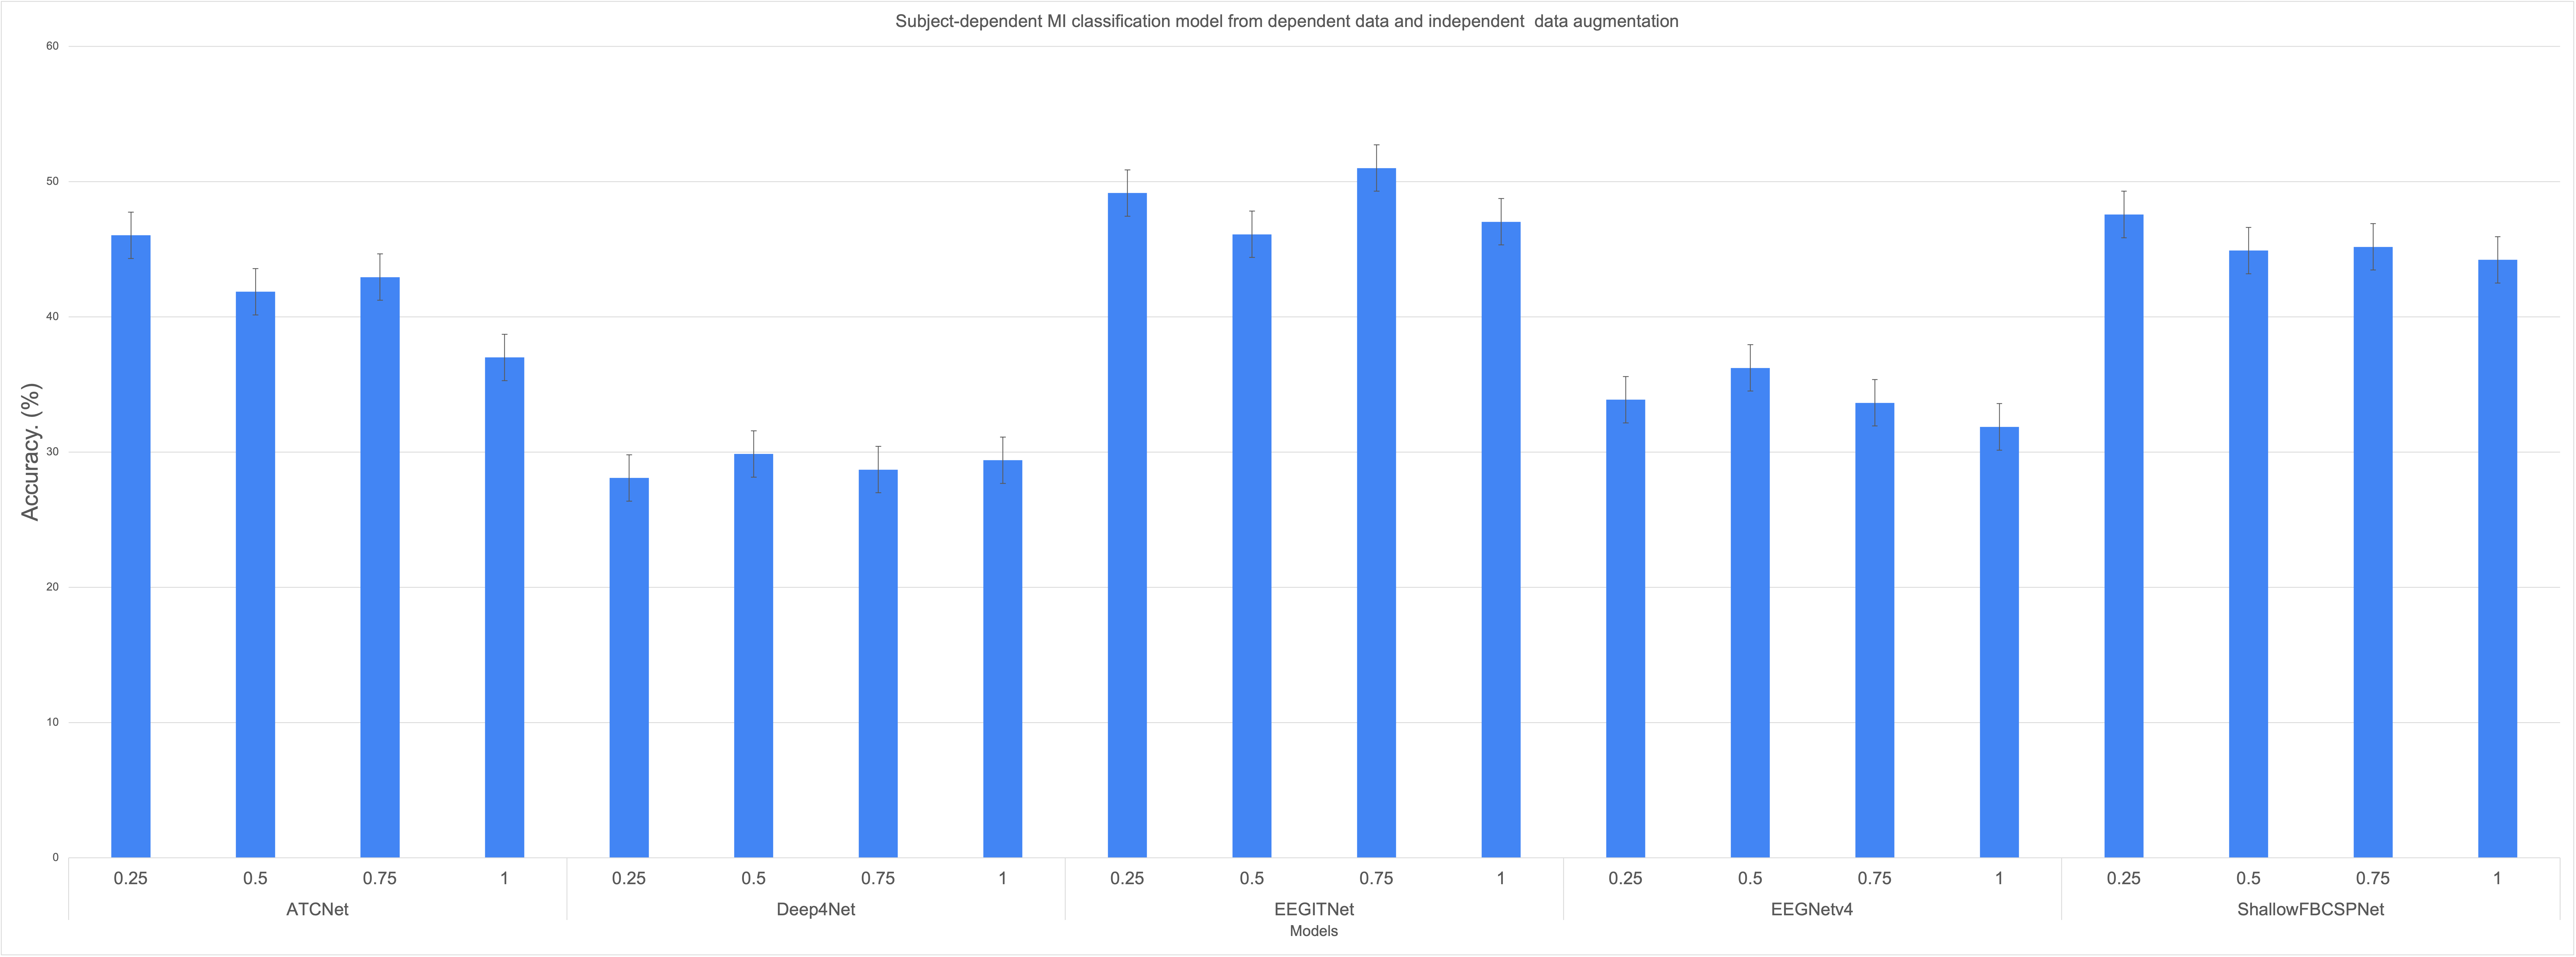
\includegraphics[width=1.1\textwidth]{fig/dependent_data_and_independent_data_augmentation.png}
  \label{fig:Subject-dependent MI classification model from dependent and independent data augmentation result}
\end{figure}

\subsection{Subject-independent MI classification model from independent data and independent synthetic data}

The Subject-dependent MI classification model accuracy trained by dependent data augmentation are displayed in figure \ref{fig:independent synthetic data}.

\begin{figure}[ht]
  \centering
  \caption[Subject-independent MI classification model from independent data and independent synthetic data result]{Subject-independent MI classification model from independent data and independent synthetic data result}
  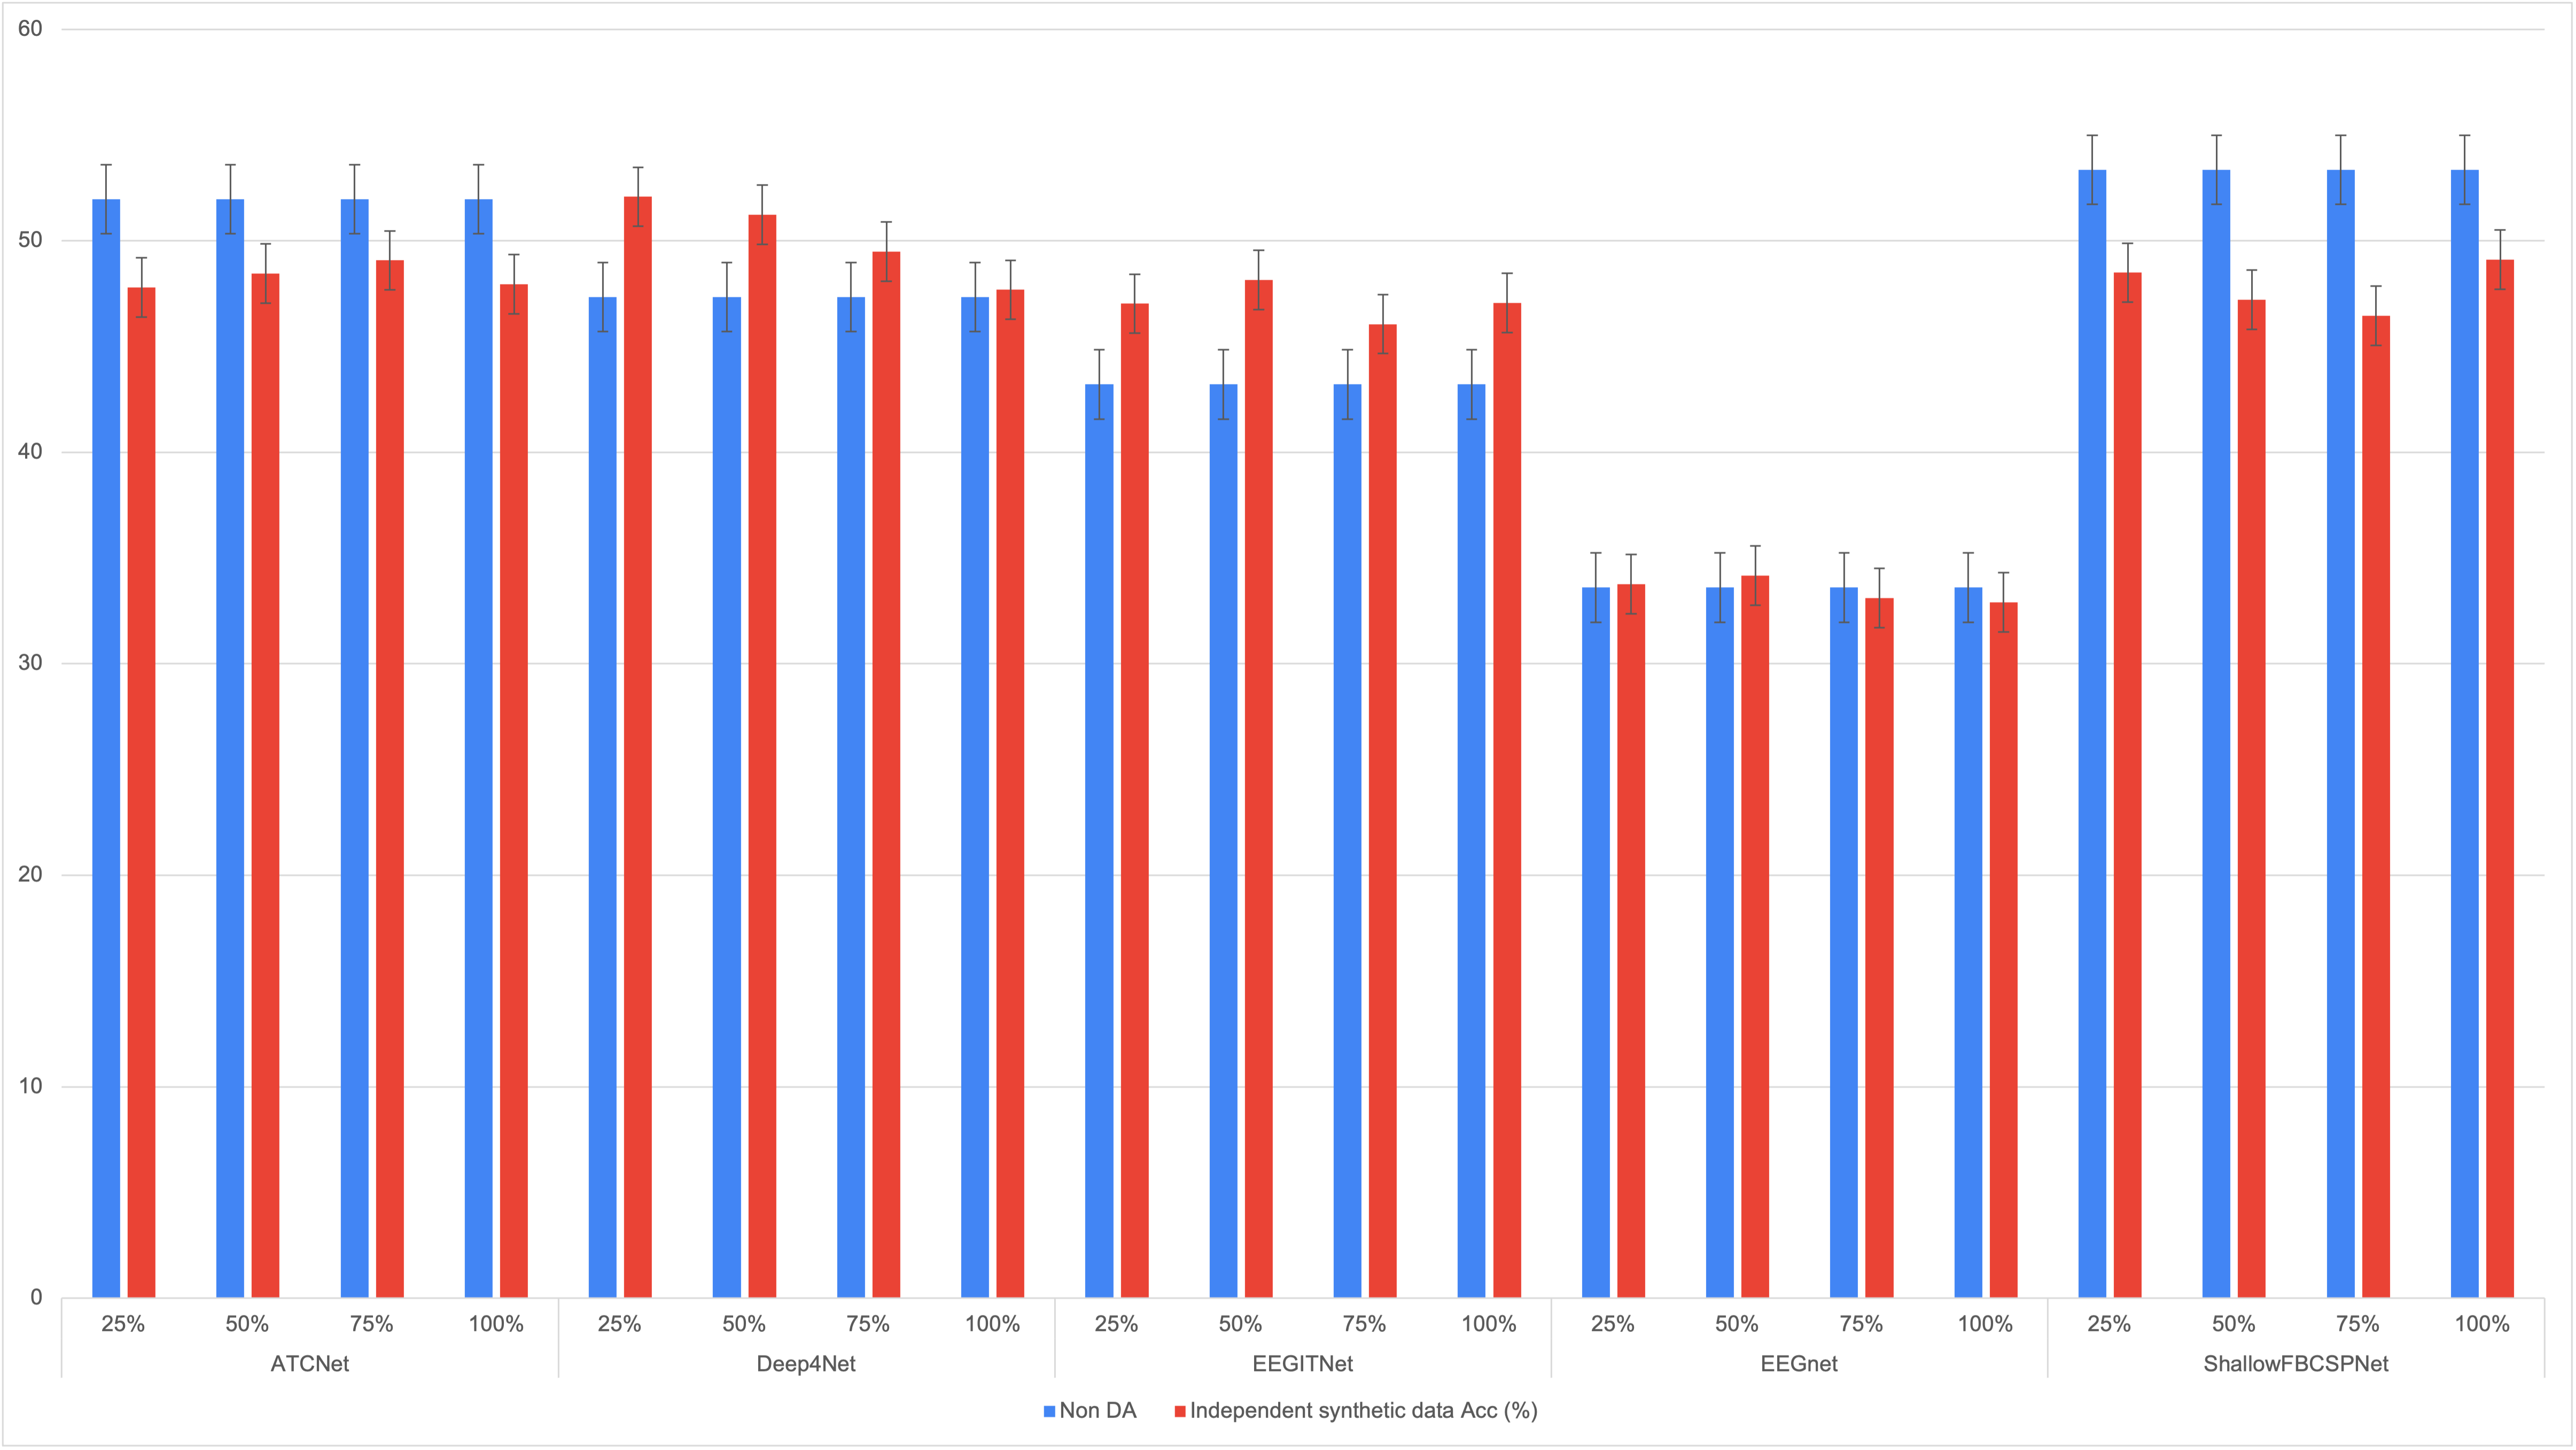
\includegraphics[width=1.1\textwidth]{fig/independent synthetic data.png.png}
  \label{fig:independent synthetic data}
\end{figure}


\subsection{Concluded All Result of Subject-dependent MI classification model}

In this section, we are displaying all the results of all methods of the subject-dependent MI classification model in figure \ref{fig:All the results of the subject-dependent MI classification model}.

\begin{figure}[ht]
  \centering
  \caption[All the results of the subject-dependent MI classification model]{All the results of the subject-dependent MI classification model}
  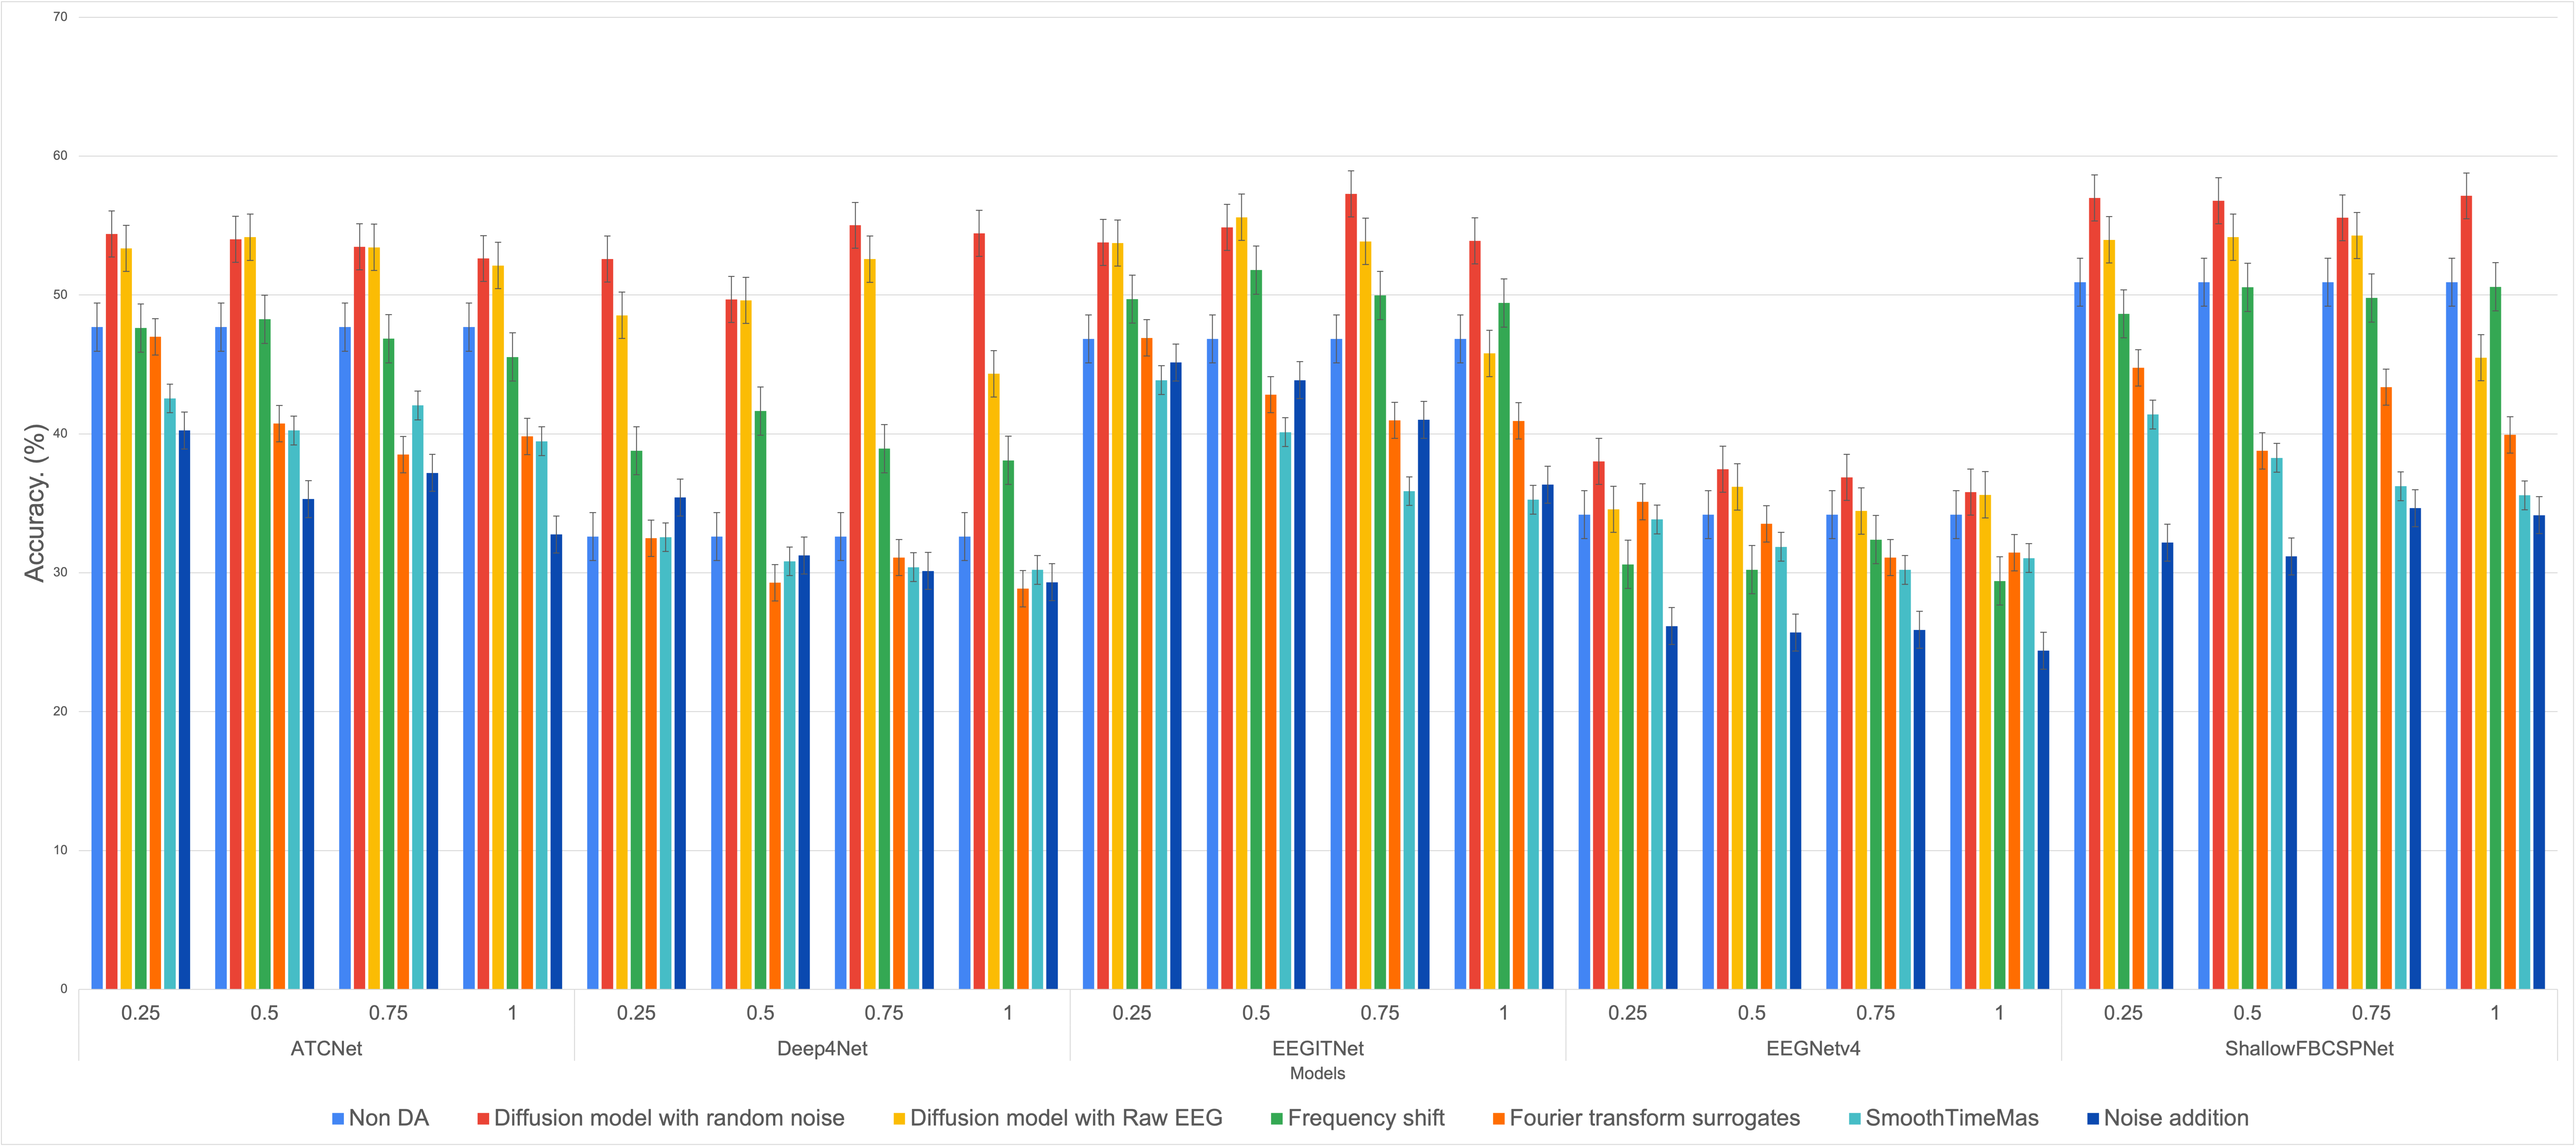
\includegraphics[width=1.1\textwidth]{fig/Con.png}
  \label{fig:All the results of the subject-dependent MI classification model}
\end{figure}


\textbf{\subsection{Baseline Accuracy}
The accuracy of the standard EEG MI classification models is considered to be the baseline accuracy. The models are ATCNet, Deep4Net, EEGITNet, EEGNet, and ShallowFBCSPNet. The baseline accuracy, which trained by only raw dataset without DA. We present the result on the table \ref{Baseline Accuracy}.
\begin{table}[ht] 
\centering
\caption{\label{Baseline Accuracy} Baseline Accuracy }
 %\caption[discussion]{Subject-dependent accuracy improvement}
%\label{table:Subject-dependent accuracy improvement}
\begin{tabular}{ll|llllllllll}
\hline
Baseline Accuracy & Size DA & WaveGrad & sigma & Noise addition & sigma & Frequency shift & sigma & Fourier transform surrogates & sigma & SmoothTimeMas & sigma \\ \hline
42.45 & 0.25 & 51.15 & 17.61 & 35.83 & 13.95 & 43.07 & 18.28 & 41.25 & 14.31 & 38.84 & 12.38 \\
      & 0.5  & 50.56 & 17.38 & 33.46 & 11.10 & 44.49 & 17.82 & 37.03 & 10.85 & 36.27 & 10.84 \\
      & 0.75 & 51.64 & 17.24 & 33.77 & 11.23 & 43.58 & 18.25 & 37.01 & 10.14 & 34.95 & 10.73 \\
      & 1    & 50.78 & 17.72 & 31.39 & 8.84  & 42.61 & 18.80 & 36.20 & 11.03 & 34.31 & 9.51  \\ \hline
\end{tabular}
\end{table}


\subsection{Implementation Synthetic Data Accuracy}

We trained standard EEG MI classification models by raw EEG data and dependent synthetic data. We created train set by stack dependent synthetic dataset and raw EEG dataset. The amount of synthetic data is 25\%, 50\%, 75\%, and 100\% of the size of raw EEG data set. The accuracy are present on the table \ref{Synthetic Data Accuracy}.
 
\begin{table}[ht] 
\centering
\caption{\label{Synthetic Data Accuracy} Synthetic Data Accuracy }
\scalebox{0.5}{
\begin{tabular}{ll|ll}
\hline
Network                & DA Size & WaveGrad Accracy & StdDev of WaveGrad \\\mr
ATCNet          & 25\%    & 54.40            & 19.09              \\
                & 50\%    & 54.01            & 18.30              \\
                & 75\%    & 53.47            & 20.65              \\
                & 100\%   & 52.62            & 19.01              \\\mr
Deep4Net        & 25\%    & 52.58            & 19.20              \\
                & 50\%    & 49.67            & 20.99              \\
                & 75\%    & 55.02            & 18.83              \\
                & 100\%   & 54.44            & 17.68              \\\mr
EEGITNet        & 25\%    & 53.78            & 17.62              \\
                & 50\%    & 54.86            & 17.13              \\
                & 75\%    & 57.29            & 15.41              \\
                & 100\%   & 53.90            & 19.46              \\\mr
EEGNet        & 25\%    & 38.03            & 9.63               \\
                & 50\%    & 37.45            & 8.58               \\
                & 75\%    & 36.86            & 8.20               \\
                & 100\%   & 35.80            & 6.57               \\\mr
ShallowFBCSPNet & 25\%    & 56.98            & 17.74              \\
                & 50\%    & 56.79            & 15.68              \\
                & 75\%    & 55.56            & 15.29              \\
                & 100\%   & 57.14            & 17.41             \\ \hline
\end{tabular}
}
\end{table}
}



\begin{table}[ht] 
\centering
\caption{\label{table:Comparing Data Augmentation Accuracy} Comparing Data Augmentation Accuracy }
\scalebox{0.5}{
\begin{tabular}{lll|l|ll|ll|ll|ll|ll}
\hline
Network &
  Baseline (\%) &
  \sigma &
  DA size &
  WaveGrad (\%) &
  \sigma &
  Noise addition (\%) &
  \sigma &
  Frequency shift (\%) &
  \sigma &
  FTSurrogate (\%) &
  \sigma &
  SmoothTimeMas (\%) &
  \sigma \\\mr
ATCNet          & 47.68 & 18.78 & 25\%  &  \textbf{54.40} & 19.09 &  \textbf{40.24} & 18.26 & 47.62 & 18.74 &  \textbf{46.99} & 18.06 &  \textbf{42.55} & 15.28 \\
                &       &       & 50\%  & 54.01 & 18.30 & 35.30 & 10.10 &  \textbf{48.26} & 19.57 & 40.74 & 12.05 & 40.24 & 12.97 \\
                &       &       & 75\%  & 53.47 & 20.65 & 37.19 & 13.69 & 46.85 & 20.18 & 38.50 & 12.79 & 42.05 & 15.33 \\
                &       &       & 100\% & 52.62 & 19.01 & 32.75 & 7.72  & 45.54 & 19.07 & 39.81 & 12.98 & 39.47 & 10.91 \\\mr
Deep4Net        & 32.60 & 16.67 & 25\%  & 52.58 & 19.20 &  \textbf{35.42} & 11.74 & 38.79 & 22.18 &  \textbf{32.48} & 11.60 &  \textbf{32.56} & 7.81  \\
                &       &       & 50\%  & 49.67 & 20.99 & 31.25 & 10.09 &  \textbf{41.64} & 17.85 & 29.28 & 7.01  & 30.83 & 7.11  \\
                &       &       & 75\%  &  \textbf{55.02} & 18.83 & 30.13 & 9.48  & 38.94 & 22.59 & 31.10 & 4.68  & 30.40 & 5.18  \\
                &       &       & 100\% & 54.44 & 17.68 & 29.32 & 6.91  & 38.09 & 21.38 & 28.86 & 5.55  & 30.21 & 5.08  \\\mr
EEGITNet        & 46.84 & 16.97 & 25\%  & 53.78 & 17.62 &  \textbf{45.14} & 16.43 & 49.70 & 17.85 &  \textbf{46.91} & 15.84 &  \textbf{43.87} & 16.90 \\
                &       &       & 50\%  & 54.86 & 17.13 & 43.87 & 15.13 &  \textbf{51.79} & 16.43 & 42.82 & 14.66 & 40.12 & 13.90 \\
                &       &       & 75\%  &  \textbf{57.29} & 15.41 & 41.01 & 11.71 & 49.97 & 16.21 & 40.97 & 10.63 & 35.88 & 13.33 \\
                &       &       & 100\% & 53.90 & 19.46 & 36.34 & 12.34 & 49.42 & 17.49 & 40.93 & 14.26 & 35.26 & 13.73 \\\mr
EEGNet        & 34.18 & 8.50  & 25\%  &  \textbf{38.03} & 9.63  &  \textbf{26.16} & 2.95  & 30.61 & 7.44  &  \textbf{35.11} & 8.66  &  \textbf{33.83} & 9.35  \\
                &       &       & 50\%  & 37.45 & 8.58  & 25.69 & 1.08  & 30.22 & 7.22  & 33.53 & 5.55  & 31.87 & 8.38  \\
                &       &       & 75\%  & 36.86 & 8.20  & 25.89 & 3.65  &  \textbf{32.38} & 7.99  & 31.10 & 5.89  & 30.21 & 6.28  \\
                &       &       & 100\% & 35.80 & 6.57  & 24.38 & 1.50  & 29.41 & 9.31  & 31.44 & 4.39  & 31.06 & 6.98  \\\mr
ShallowFBCSPNet & 50.93 & 16.64 & 25\%  & 56.98 & 17.74 & 32.18 & 8.97  & 48.64 & 17.83 &  \textbf{44.75} & 11.12 &  \textbf{41.40} & 7.13  \\
                &       &       & 50\%  & 56.79 & 15.68 & 31.17 & 6.21  & 50.55 & 19.16 & 38.77 & 8.36  & 38.27 & 8.37  \\
                &       &       & 75\%  & 55.56 & 15.29 &  \textbf{34.65} & 10.39 & 49.78 & 17.93 & 43.36 & 9.37  & 36.23 & 6.84  \\
                &       &       & 100\% &  \textbf{57.14} & 17.41 & 34.14 & 8.36  &  \textbf{50.59} & 19.44 & 39.93 & 10.26 & 35.57 & 7.16  \\\hline
\end{tabular}}
\end{table}



\begin{table}[ht] 
\centering
\caption{\label{table: Success subjects Accuracy} Success subjects Accuracy }
\scalebox{0.6}{
 %\caption[discussion]{Subject-dependent accuracy improvement}
%\label{table:Subject-dependent accuracy improvement}
\begin{tabular}{lll|l|lllll}
\hline
Subject Number & Model & Baseline (\%) & DA size & WaveGrad & Noise addition (\%) & Frequency shift (\%) & FTSurrogate (\%) & SmoothTimeMas (\%) \\\mr
\textbf{3} & ATCNet          & 69.10 & 25\%  & 75.35 & 68.40 & 70.31 & 70.49 & 68.06 \\
  &                 &       & 50\%  & 75.69 & 30.90 & 72.39 & 58.33 & 46.53 \\
  &                 &       & 75\%  & 80.56 & 63.54 & 69.61 & 57.99 & 57.99 \\
  &                 &       & 100\% & 71.18 & 35.42 & 62.67 & 54.86 & 42.01 \\\cline{2-9}
  & Deep4Net        & 26.74 & 25\%  & 73.26 & 39.24 & 65.79 & 36.81 & 31.60 \\
  &                 &       & 50\%  & 75.35 & 35.42 & 28.99 & 29.17 & 40.63 \\
  &                 &       & 75\%  & 76.74 & 30.90 & 71.35 & 32.99 & 33.33 \\
  &                 &       & 100\% & 77.78 & 35.76 & 32.11 & 26.39 & 31.94 \\\cline{2-9}
  & EEGITNet        & 70.14 & 25\%  & 77.43 & 63.19 & 72.04 & 64.58 & 64.58 \\
  &                 &       & 50\%  & 76.04 & 67.71 & 79.68 & 61.11 & 46.88 \\
  &                 &       & 75\%  & 82.29 & 57.64 & 74.82 & 56.94 & 52.43 \\
  &                 &       & 100\% & 87.50 & 60.42 & 74.47 & 60.76 & 46.18 \\\cline{2-9}
  & EEGNet          & 43.75 & 25\%  & 53.47 & 25.00 & 41.14 & 43.40 & 47.57 \\
  &                 &       & 50\%  & 49.31 & 25.00 & 34.54 & 40.63 & 41.67 \\
  &                 &       & 75\%  & 53.47 & 25.00 & 37.32 & 35.42 & 38.89 \\
  &                 &       & 100\% & 44.10 & 25.00 & 30.72 & 35.42 & 35.42 \\\cline{2-9}
  & ShallowFBCSPNet & 75.00 & 25\%  & 81.94 & 33.33 & 74.82 & 57.64 & 50.69 \\
  &                 &       & 50\%  & 78.82 & 38.54 & 72.74 & 46.18 & 46.53 \\
  &                 &       & 75\%  & 77.78 & 56.60 & 72.74 & 53.82 & 45.49 \\
  &                 &       & 100\% & 78.13 & 35.76 & 76.56 & 48.96 & 34.38 \\\mr
\textbf{9} & ATCNet          & 69.10 & 25\%  & 77.43 & 52.08 & 69.26 & 64.93 & 60.76 \\
  &                 &       & 50\%  & 72.22 & 46.53 & 64.75 & 52.08 & 64.24 \\
  &                 &       & 75\%  & 75.69 & 53.47 & 70.31 & 51.39 & 61.11 \\
  &                 &       & 100\% & 75.69 & 38.89 & 63.71 & 57.29 & 52.43 \\\cline{2-9}
  & Deep4Net        & 26.74 & 25\%  & 73.61 & 45.49 & 71.69 & 61.46 & 48.96 \\
  &                 &       & 50\%  & 75.00 & 48.96 & 66.49 & 46.88 & 42.36 \\
  &                 &       & 75\%  & 75.35 & 45.49 & 71.35 & 41.67 & 41.67 \\
  &                 &       & 100\% & 73.96 & 43.06 & 69.96 & 41.67 & 42.01 \\\cline{2-9}
  & EEGITNet        & 70.14 & 25\%  & 72.92 & 64.58 & 65.79 & 67.71 & 65.28 \\
  &                 &       & 50\%  & 76.04 & 58.68 & 71.69 & 53.13 & 55.90 \\
  &                 &       & 75\%  & 71.88 & 53.47 & 68.92 & 55.21 & 41.67 \\
  &                 &       & 100\% & 72.92 & 47.22 & 71.35 & 51.74 & 52.78 \\\cline{2-9}
  & EEGNet          & 43.75 & 25\%  & 53.13 & 25.00 & 43.22 & 51.39 & 49.65 \\
  &                 &       & 50\%  & 50.35 & 25.00 & 43.92 & 43.75 & 48.96 \\
  &                 &       & 75\%  & 44.79 & 35.07 & 51.21 & 43.75 & 41.32 \\
  &                 &       & 100\% & 46.53 & 25.00 & 51.56 & 36.46 & 45.83 \\\cline{2-9}
  & ShallowFBCSPNet & 75.00 & 25\%  & 72.57 & 55.21 & 61.28 & 60.42 & 46.18 \\
  &                 &       & 50\%  & 65.97 & 37.50 & 67.18 & 51.74 & 46.88 \\
  &                 &       & 75\%  & 70.49 & 43.40 & 63.36 & 57.99 & 39.93 \\
  &                 &       & 100\% & 70.49 & 53.47 & 64.06 & 58.68 & 45.14 \\\mr
\end{tabular}}
\end{table}

\begin{table}[ht] 
\centering
\caption{\label{table: Success subjects Accuracy} Success Subjects Accuracy Improvement }
\scalebox{0.45}{
 %\caption[discussion]{Subject-dependent accuracy improvement}
%\label{table:Subject-dependent accuracy improvement}
\begin{tabular}{lll|lllll} \mr
Subject Number &
  Network &
  DA size &
  \Delta Accuracy of  WaveGrad (\%) &
  \Delta Accuracy of   Noise addition (\%) &
  \Delta Accuracy of  Frequency shift (\%) &
  \Delta Accuracy of  FTSurrogate (\%) &
  \Delta Accuracy of  SmoothTimeMas (\%) \\\mr
\textbf{3} & ATCNet          & 25\%  & 31.95 & 25.00  & 26.91  & 27.09  & 24.66  \\
  &                 & 50\%  & 32.29 & -12.50 & 28.99  & 14.93  & 3.13   \\
  &                 & 75\%  & \textbf{37.16} & 20.14  & 26.21  & 14.59  & 14.59  \\
  &                 & 100\% & 27.78 & -7.98  & 19.27  & 11.46  & -1.39  \\\cline{2-8}
  & Deep4Net        & 25\%  & 29.86 & -4.16  & 22.39  & -6.59  & -11.80 \\
  &                 & 50\%  & 31.95 & -7.98  & -14.41 & -14.23 & -2.78  \\
  &                 & 75\%  & 33.34 & -12.50 & 27.95  & -10.41 & -10.07 \\
  &                 & 100\% & \textbf{34.38} & -7.64  & -11.29 & -17.01 & -11.46 \\\cline{2-8}
  & EEGITNet        & 25\%  & 29.86 & -4.16  & 22.39  & -6.59  & -11.80 \\
  &                 & 50\%  & 31.95 & -7.98  & -14.41 & -14.23 & -2.78  \\
  &                 & 75\%  & 33.34 & -12.50 & 27.95  & -10.41 & -10.07 \\
  &                 & 100\% & \textbf{34.38} & -7.64  & -11.29 & -17.01 & -11.46 \\\cline{2-8}
  & EEGNet          & 25\%  & 34.03 & 19.79  & 28.64  & 21.18  & 21.18  \\
  &                 & 50\%  & 32.64 & 24.31  & 36.28  & 17.71  & 3.48   \\
  &                 & 75\%  & 38.89 & 14.24  & 31.42  & 13.54  & 9.03   \\
  &                 & 100\% & \textbf{44.10} & 17.02  & 31.07  & 17.36  & 2.78   \\\cline{2-8}
  & ShallowFBCSPNet & 25\%  & \textbf{38.54} & -10.07 & 31.42  & 14.24  & 7.29   \\
  &                 & 50\%  & 35.42 & -4.86  & 29.34  & 2.78   & 3.13   \\
  &                 & 75\%  & 34.38 & 13.20  & 29.34  & 10.42  & 2.09   \\
  &                 & 100\% & 34.73 & -7.64  & 33.16  & 5.56   & -9.03  \\\mr
\textbf{9} & ATCNet          & 25\%  & 34.03 & 8.68   & 25.86  & 21.53  & 17.36  \\
  &                 & 50\%  & 28.82 & 3.13   & 21.35  & 8.68   & 20.84  \\
  &                 & 75\%  & 32.29 & 10.07  & 26.91  & 7.99   & 17.71  \\
  &                 & 100\% & 32.29 & -4.51  & 20.31  & 13.89  & 9.03   \\\cline{2-8}
  & Deep4Net        & 25\%  & 30.21 & 2.09   & 28.29  & 18.06  & 5.56   \\
  &                 & 50\%  & 31.60 & 5.56   & 23.09  & 3.48   & -1.04  \\
  &                 & 75\%  & 31.95 & 2.09   & 27.95  & -1.73  & -1.73  \\
  &                 & 100\% & 30.56 & -0.34  & 26.56  & -1.73  & -1.39  \\\cline{2-8}
  & EEGITNet        & 25\%  & 29.52 & 21.18  & 22.39  & 24.31  & 21.88  \\
  &                 & 50\%  & 32.64 & 15.28  & 28.29  & 9.73   & 12.50  \\
  &                 & 75\%  & 28.48 & 10.07  & 25.52  & 11.81  & -1.73  \\
  &                 & 100\% & 29.52 & 3.82   & 27.95  & 8.34   & 9.38   \\\cline{2-8}
  & EEGNet          & 25\%  & 9.73  & -18.40 & -0.18  & 7.99   & 6.25   \\
  &                 & 50\%  & 6.95  & -18.40 & 0.52   & 0.35   & 5.56   \\
  &                 & 75\%  & 1.39  & -8.33  & 7.81   & 0.35   & -2.08  \\
  &                 & 100\% & 3.13  & -18.40 & 8.16   & -6.94  & 2.43   \\\cline{2-8}
  & ShallowFBCSPNet & 25\%  & 29.17 & 11.81  & 17.88  & 17.02  & 2.78   \\
  &                 & 50\%  & 22.57 & -5.90  & 23.78  & 8.34   & 3.48   \\
  &                 & 75\%  & 27.09 & 0.00   & 19.96  & 14.59  & -3.47  \\
  &                 & 100\% & 27.09 & 10.07  & 20.66  & 15.28  & 1.74   \\ \mr
\end{tabular}}
\end{table}





\begin{table}[ht] 
\centering
\caption{\label{table: ineffective subjects Accuracy} Unsuccessful subjects Accuracy}
\scalebox{0.6}{\begin{tabular}{lll|l|lllll}
\mr
Subject Number & Network & Baseline (\%) & DA size & WaveGrad & Noise addition (\%) & Frequency shift (\%) & FTSurrogate (\%) & SmoothTimeMas (\%) \\ \mr
\textbf{2} & ATCNet          & 24.31 & 25\%  & 36.46 & 29.86 & 29.33 & 30.90 & 24.31 \\
  &                 &       & 50\%  & 37.15 & 25.00 & 27.94 & 26.04 & 27.43 \\
  &                 &       & 75\%  & 30.56 & 27.08 & 26.56 & 25.00 & 26.04 \\
  &                 &       & 100\% & 27.78 & 23.61 & 29.33 & 23.96 & 25.00 \\\cline{2-9}
  & Deep4Net        & 35.07 & 25\%  & 37.50 & 24.65 & 20.31 & 26.39 & 28.47 \\
  &                 &       & 50\%  & 36.64 & 24.31 & 21.00 & 27.08 & 24.31 \\
  &                 &       & 75\%  & 37.50 & 22.22 & 19.96 & 29.17 & 24.31 \\
  &                 &       & 100\% & 38.54 & 23.26 & 25.86 & 24.31 & 26.04 \\\cline{2-9}
  & EEGITNet        & 28.47 & 25\%  & 32.64 & 22.22 & 30.72 & 30.90 & 25.35 \\
  &                 &       & 50\%  & 38.89 & 29.51 & 32.81 & 22.22 & 29.51 \\
  &                 &       & 75\%  & 42.71 & 25.00 & 35.58 & 32.64 & 24.31 \\
  &                 &       & 100\% & 41.32 & 26.04 & 35.93 & 25.35 & 24.31 \\\cline{2-9}
  & EEGNet          & 25.00 & 25\%  & 27.08 & 25.00 & 22.04 & 22.57 & 26.74 \\
  &                 &       & 50\%  & 27.08 & 26.39 & 24.47 & 29.86 & 25.35 \\
  &                 &       & 75\%  & 26.92 & 22.92 & 25.51 & 26.39 & 22.57 \\
  &                 &       & 100\% & 28.82 & 21.53 & 19.26 & 29.17 & 27.08 \\\cline{2-9}
  & ShallowFBCSPNet & 33.33 & 25\%  & 38.89 & 28.47 & 28.99 & 28.47 & 30.56 \\
  &                 &       & 50\%  & 42.71 & 29.51 & 30.38 & 27.78 & 25.35 \\
  &                 &       & 75\%  & 44.10 & 25.69 & 30.03 & 32.99 & 31.60 \\
  &                 &       & 100\% & 40.62 & 27.43 & 31.07 & 28.82 & 24.65 \\\mr
\textbf{5} & ATCNet          & 27.08 & 25\%  & 29.51 & 25.69 & 26.21 & 25.35 & 28.82 \\
  &                 &       & 50\%  & 28.13 & 28.13 & 21.53 & 28.47 & 25.00 \\
  &                 &       & 75\%  & 27.43 & 26.04 & 24.82 & 23.26 & 25.00 \\
  &                 &       & 100\% & 29.86 & 24.65 & 18.92 & 23.26 & 25.35 \\\cline{2-9}
  & Deep4Net        & 25    & 25\%  & 27.43 & 22.92 & 20.31 & 26.04 & 25.00 \\
  &                 &       & 50\%  & 31.25 & 20.83 & 23.08 & 24.31 & 28.82 \\
  &                 &       & 75\%  & 28.47 & 23.61 & 19.26 & 26.39 & 25.35 \\
  &                 &       & 100\% & 27.78 & 25.00 & 18.22 & 25.00 & 28.13 \\\cline{2-9}
  & EEGITNet        & 27.78 & 25\%  & 34.03 & 25.00 & 25.86 & 34.38 & 29.86 \\
  &                 &       & 50\%  & 32.64 & 28.13 & 37.67 & 27.78 & 27.43 \\
  &                 &       & 75\%  & 39.58 & 28.82 & 29.68 & 24.31 & 23.61 \\
  &                 &       & 100\% & 31.94 & 28.13 & 30.03 & 26.74 & 24.31 \\\cline{2-9}
  & EEGNet          & 24.31 & 25\%  & 31.60 & 25.00 & 25.17 & 27.78 & 25.69 \\
  &                 &       & 50\%  & 28.47 & 25.35 & 19.96 & 27.43 & 24.31 \\
  &                 &       & 75\%  & 30.90 & 23.96 & 26.56 & 25.35 & 31.25 \\
  &                 &       & 100\% & 28.47 & 23.26 & 24.82 & 25.69 & 27.78 \\\cline{2-9}
  & ShallowFBCSPNet & 31.25 & 25\%  & 35.07 & 27.43 & 22.47 & 30.56 & 34.38 \\
  &                 &       & 50\%  & 32.99 & 25.69 & 26.21 & 28.47 & 27.08 \\
  &                 &       & 75\%  & 35.42 & 28.47 & 26.21 & 36.46 & 30.56 \\
  &                 &       & 100\% & 33.33 & 30.21 & 21.69 & 29.51 & 26.39 \\\mr
   
\end{tabular}}
\end{table}


\begin{table}[ht] 
\centering
\caption{\label{table: ineffective Subjects Accuracy Change } Unsuccess Subjects Accuracy Change }
\scalebox{0.45}{\begin{tabular}{lll|lllll}\mr
Subject Number &
  Network &
  DA size &
  \Delta Accuracy of  WaveGrad (\%) &
  \Delta Accuracy of   Noise addition (\%) &
  \Delta Accuracy of  Frequency shift (\%) &
  \Delta Accuracy of  FTSurrogate (\%) &
  \Delta Accuracy of  SmoothTimeMas (\%) &
   \\\mr
\textbf{2} & ATCNet          & 25\% & 12.15  & 5.56   & 5.02   & 6.60   & 0.00   &  \\
  &                 & 50\%  & 37.15  & 25.00  & 27.94  & 26.04  & 27.43  &  \\
  &                 & 75\% & 30.56  & 27.08  & 26.56  & 25.00  & 26.04  &  \\
  &                 & 100\%    & 27.78  & 23.61  & 29.33  & 23.96  & 25.00  &  \\\cline{2-8}
  & Deep4Net        & 25\% & 13.54  & 0.69   & -3.65  & 2.43   & 4.51   &  \\
  &                 & 50\%  & 12.68  & 0.35   & -2.96  & 3.12   & 0.35   &  \\
  &                 & 75\% & 13.54  & -1.74  & -4.00  & 5.21   & 0.35   &  \\
  &                 & 100\%    & 14.58  & -0.70  & 1.90   & 0.35   & 2.08   &  \\\cline{2-8}
  & EEGITNet        & 25\% & -22.22 & -32.64 & -24.14 & -23.96 & -29.51 &  \\
  &                 & 50\%  & -15.97 & -25.35 & -22.05 & -32.64 & -25.35 &  \\
  &                 & 75\% & -12.15 & -29.86 & -19.28 & -22.22 & -30.55 &  \\
  &                 & 100\%    & -13.54 & -28.82 & -18.93 & -29.51 & -30.55 &  \\\cline{2-8}
  & EEGNet          & 25\%& -7.30  & -9.38  & -12.34 & -11.81 & -7.64  &  \\
  &                 & 50\%  & -7.30  & -7.99  & -9.91  & -4.52  & -9.03  &  \\
  &                 & 75\% & -7.46  & -11.46 & -8.87  & -7.99  & -11.81 &  \\
  &                 & 100\%    & -5.56  & -12.85 & -15.12 & -5.21  & -7.30  &  \\\cline{2-8}
  & ShallowFBCSPNet & 25\% & -19.79 & -30.21 & -29.69 & -30.21 & -28.13 &  \\
  &                 & 50\%  & -15.97 & -29.17 & -28.30 & -30.90 & -33.33 &  \\
  &                 & 75\% & -14.58 & -32.99 & -28.65 & -25.69 & -27.08 &  \\
  &                 & 100\%    & -18.06 & -31.25 & -27.61 & -29.86 & -34.03 &  \\\mr
\textbf{5} & ATCNet          & 25\% & -13.89 & -17.71 & -17.19 & -18.05 & -14.58 &  \\
  &                 & 50\%  & -15.28 & -15.28 & -21.87 & -14.93 & -18.40 &  \\
  &                 & 75\% & -15.97 & -17.36 & -18.58 & -20.14 & -18.40 &  \\
  &                 & 100\%    & -13.54 & -18.75 & -24.48 & -20.14 & -18.05 &  \\\cline{2-8}
  & Deep4Net        & 25\% & -15.97 & -20.48 & -23.09 & -17.36 & -18.40 &  \\
  &                 & 50\%  & -12.15 & -22.57 & -20.32 & -19.09 & -14.58 &  \\
  &                 & 75\% & -14.93 & -19.79 & -24.14 & -17.01 & -18.05 &  \\
  &                 & 100\%    & -15.62 & -18.40 & -25.18 & -18.40 & -15.28 &  \\\cline{2-8}
  & EEGITNet        & 25\% & -9.37  & -18.40 & -17.54 & -9.03  & -13.54 &  \\
  &                 & 50\%  & -10.76 & -15.28 & -5.73  & -15.62 & -15.97 &  \\
  &                 & 75\% & -3.82  & -14.58 & -13.72 & -19.09 & -19.79 &  \\
  &                 & 100\%    & -11.46 & -15.28 & -13.37 & -16.66 & -19.09 &  \\\cline{2-8}
  & EEGNet          & 25\% & -11.80 & -18.40 & -18.23 & -15.62 & -17.71 &  \\
  &                 & 50\%  & -14.93 & -18.05 & -23.44 & -15.97 & -19.09 &  \\
  &                 & 75\% & -12.50 & -19.44 & -16.84 & -18.05 & -12.15 &  \\
  &                 & 100\%    & -14.93 & -20.14 & -18.58 & -17.71 & -15.62 &  \\\cline{2-8}
  & ShallowFBCSPNet & 25\% & -8.33  & -15.97 & -20.93 & -12.84 & -9.03  &  \\
  &                 & 50\%  & -10.41 & -17.71 & -17.19 & -14.93 & -16.32 &  \\
  &                 & 75\% & -7.98  & -14.93 & -17.19 & -6.94  & -12.84 &  \\
  &                 & 100\%    & -10.07 & -13.19 & -21.71 & -13.89 & -17.01 &  \mr

\end{tabular}}
\end{table}



\begin{tabular}{ll|lllll}
\mr
Subject Number &
  DA size &
  \Delta of  WaveGrad (\%) &
  \Delta of   Noise addition (\%) &
  \Delta of  Frequency shift (\%) &
  \Delta of  FTSurrogate (\%) &
  \Delta of  SmoothTimeMas (\%) \\\mr
1 & 25\%  & 16.88 & -0.28  & 2.32  & 0.83   & 4.72   \\
  & 50\%  & 18.33 & -0.49  & 11.21 & -0.07  & -2.43  \\
  & 75\%  & 18.33 & -4.86  & 9.12  & -1.95  & -1.60  \\
  & 100\% & 14.51 & -11.53 & 10.72 & -0.42  & -0.70  \\\mr
2 & 25\%  & 5.28  & -3.19  & -2.96 & -1.39  & -2.15  \\
  & 50\%  & 7.26  & -2.29  & -1.92 & -2.64  & -2.85  \\
  & 75\%  & 7.12  & -4.65  & -1.71 & 0.00   & -3.47  \\
  & 100\% & 6.18  & -4.86  & -0.95 & -2.92  & -3.82  \\\mr
3 & 25\%  & 15.34 & -11.11 & 7.87  & -2.36  & -4.45  \\
  & 50\%  & 14.10 & -17.43 & 0.72  & -9.86  & -12.50 \\
  & 75\%  & 17.22 & -10.21 & 8.22  & -9.51  & -11.32 \\
  & 100\% & 14.79 & -18.47 & -1.64 & -11.67 & -18.96 \\\mr
4 & 25\%  & 5.11  & -6.67  & -0.94 & 1.11   & -1.53  \\
  & 50\%  & 8.18  & -10.14 & -0.45 & -2.50  & -3.33  \\
  & 75\%  & 9.59  & -7.64  & -2.26 & -2.29  & -4.03  \\
  & 100\% & 8.20  & -7.22  & -1.57 & -1.94  & -5.21  \\\mr
5 & 25\%  & 4.44  & -1.88  & -3.08 & 1.74   & 1.67   \\
  & 50\%  & 3.61  & -1.46  & -1.39 & 0.21   & -0.56  \\
  & 75\%  & 5.28  & -0.90  & -1.78 & 0.07   & 0.07   \\
  & 100\% & 3.19  & -0.83  & -4.35 & -1.04  & -0.70  \\\mr
6 & 25\%  & 3.68  & -2.15  & -1.15 & 0.56   & 0.97   \\
  & 50\%  & 3.89  & -0.69  & 0.38  & -1.53  & -0.42  \\
  & 75\%  & 4.65  & -4.24  & -1.85 & 0.49   & -3.13  \\
  & 100\% & 3.82  & -2.36  & -3.88 & 0.69   & -1.53  \\\mr
7 & 25\%  & 14.51 & -10.21 & 2.20  & -1.94  & -9.24  \\
  & 50\%  & 6.81  & -12.50 & 8.36  & -4.58  & -10.56 \\
  & 75\%  & 12.43 & -9.31  & 3.22  & -5.76  & -10.49 \\
  & 100\% & 13.33 & -13.68 & 0.65  & -10.63 & -10.63 \\\mr
8 & 25\%  & 8.96  & -6.81  & 4.89  & -4.72  & -10.83 \\
  & 50\%  & 8.68  & -13.47 & 4.47  & -11.53 & -8.89  \\
  & 75\%  & 6.25  & -16.67 & -1.99 & -14.24 & -12.85 \\
  & 100\% & 8.82  & -16.32 & 4.12  & -11.74 & -13.54 \\\mr
9 & 25\%  & 4.17  & -17.29 & -3.52 & -4.58  & -11.60 \\
  & 50\%  & 2.15  & -22.43 & -2.96 & -16.25 & -14.10 \\
  & 75\%  & 1.87  & -19.58 & -0.73 & -15.76 & -20.63 \\
  & 100\% & 2.15  & -24.24 & -1.64 & -16.60 & -18.13 \\\mr
\end{tabular}



\begin{tabular}{l|l|lllll}
\mr
Subjects &  Baseline Accuracy &\begin{math} \Delta \end{math} of WaveGrad & \begin{math} \Delta \end{math} of Noise addition & \begin{math} \Delta \end{math} of Frequency shift & \begin{math} \Delta \end{math} of FTSurrogate & \begin{math} \Delta \end{math} of SmoothTimeMask \\\mr
1 & 43.06 & 17.01 & -4.29  & 8.34  & -0.40  & 0.00   \\
2 & 29.24 & 6.46  & -3.75  & -1.88 & -1.74  & -3.07  \\
3 & 56.95 & 15.36 & -14.31 & 3.80  & -8.35  & -11.81 \\
4 & 37.08 & 7.77  & -7.92  & -1.31 & -1.40  & -3.52  \\
5 & 27.08 & 4.13  & -1.27  & -2.65 & 0.24   & 0.12   \\
6 & 29.58 & 4.01  & -2.36  & -1.63 & 0.05   & -1.02  \\
7 & 40.07 & 11.77 & -11.42 & 3.61  & -5.73  & -10.23 \\
8 & 53.19 & 8.18  & -13.32 & 2.87  & -10.56 & -11.53 \\
9 & 65.76 & 2.59  & -20.89 & -2.21 & -13.30 & -16.11 \\ \mr
\end{tabular}